\documentclass[nooutcomes]{ximera}
%% handout
%% space
%% newpage
%% numbers
%% nooutcomes

%I added the commands here so that I would't have to keep looking them up
%\newcommand{\RR}{\mathbb R}
%\renewcommand{\d}{\,d}
%\newcommand{\dd}[2][]{\frac{d #1}{d #2}}
%\renewcommand{\l}{\ell}
%\newcommand{\ddx}{\frac{d}{dx}}
%\everymath{\displaystyle}
%\newcommand{\dfn}{\textbf}
%\newcommand{\eval}[1]{\bigg[ #1 \bigg]}

%\begin{image}
%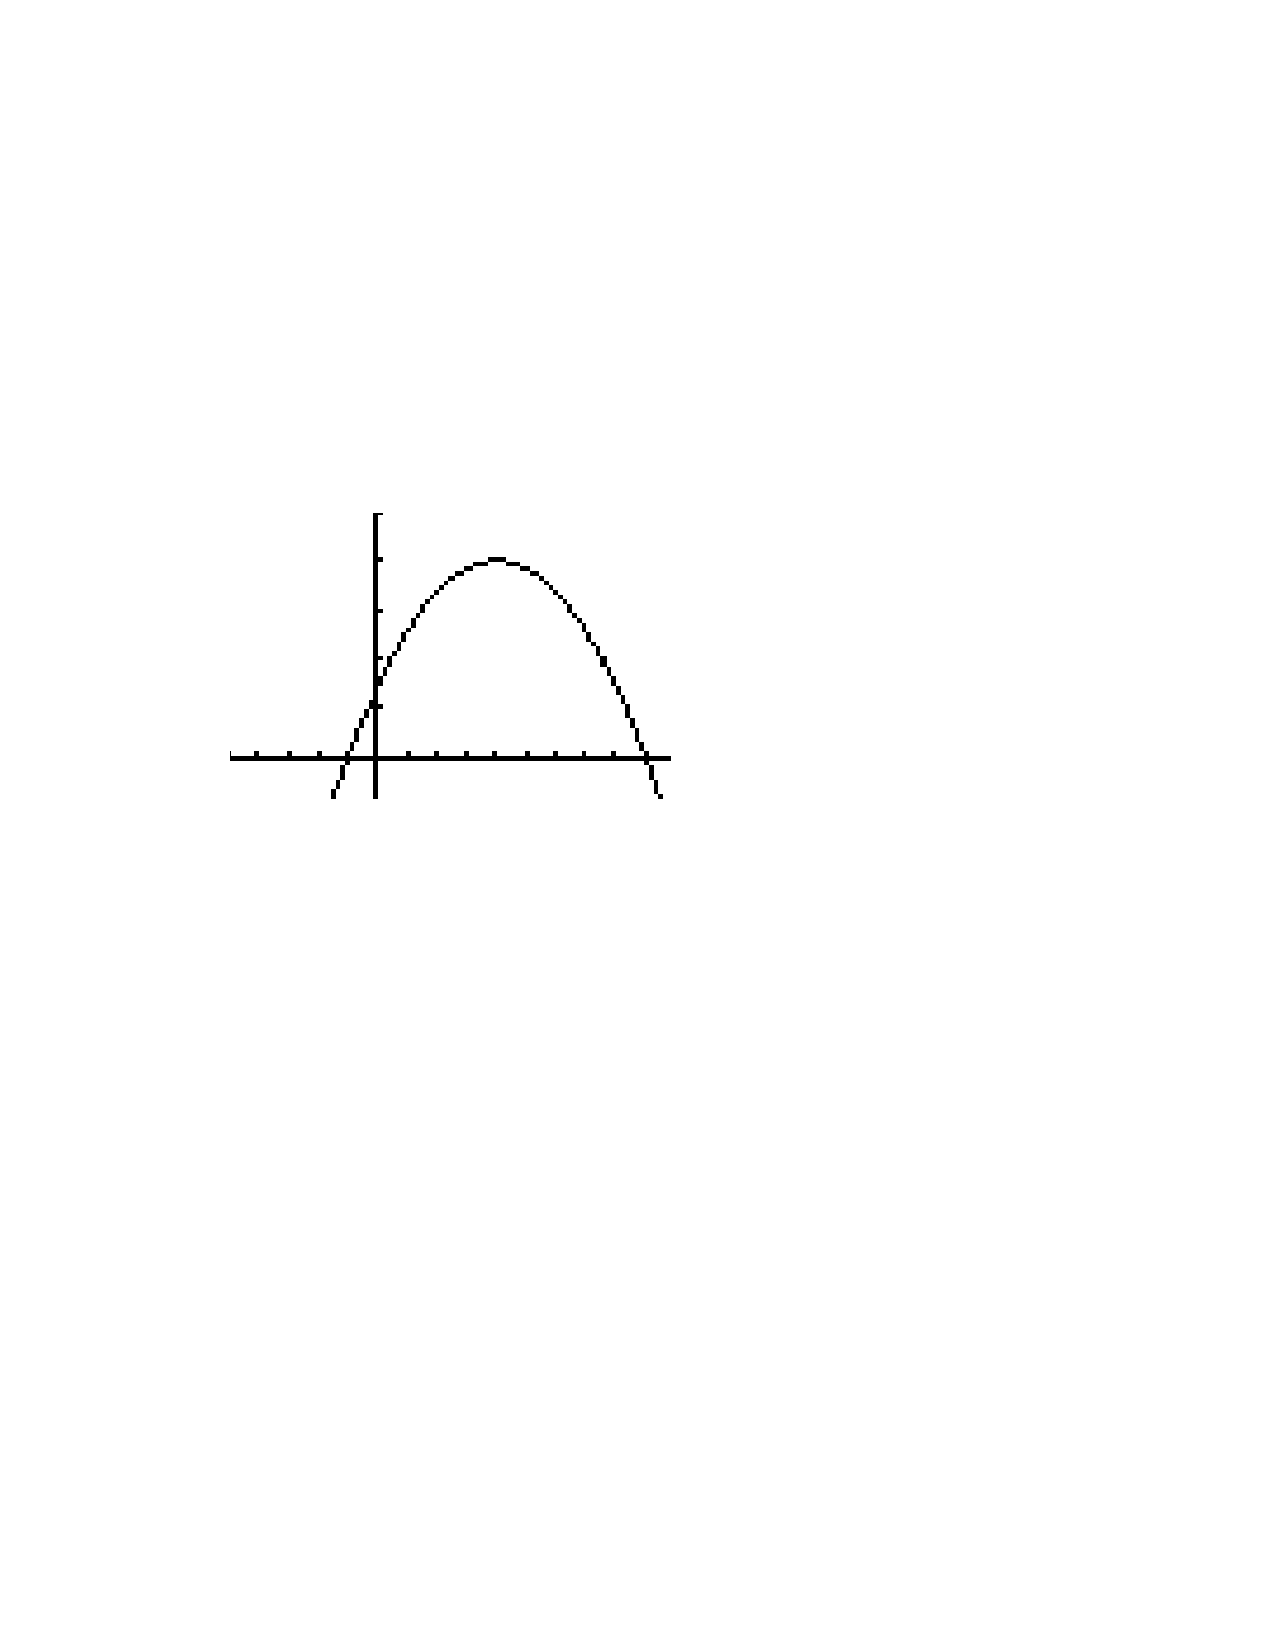
\includegraphics[trim= 170 420 250 180]{Figure1.pdf}
%\end{image}


\newcommand{\RR}{\mathbb R}
\renewcommand{\d}{\,d}
\newcommand{\dd}[2][]{\frac{d #1}{d #2}}
\renewcommand{\l}{\ell}
\newcommand{\ddx}{\frac{d}{dx}}
\newcommand{\dfn}{\textbf}
\newcommand{\eval}[1]{\bigg[ #1 \bigg]}

\usepackage{multicol}

\renewenvironment{freeResponse}{
\ifhandout\setbox0\vbox\bgroup\else
\begin{trivlist}\item[\hskip \labelsep\bfseries Solution:\hspace{2ex}]
\fi}
{\ifhandout\egroup\else
\end{trivlist}
\fi} %% we can turn off input when making a master document

\title{Recitation \#21 - 4.7 L'Hospital's Rule and 4.9 Antiderivatives (Solutions)}  

\begin{document}
\begin{abstract}		\end{abstract}
\maketitle

\section*{Warm up:} 
True or False:  You can use L'Hospital's Rule to compute $\lim_{x \to 0} \frac{|x|}{x}$ ?
		\begin{freeResponse}
		False.  The function $|x|$ is not differentiable at $x=0$, and so L'Hospital's Rule is not applicable.
		\end{freeResponse}	
		
		
		

	
	
	
	
	

\section*{Group work:}



%problem 1
\begin{problem}
State the form of each of the following limits.  If possible, state the answer to the limit based on the form.  Do not do any algebra to change the form.  If the form is indeterminate, just say it is indeterminate.
	\begin{enumerate}
	%part a
	\item  $\lim_{x \to \infty}\left( \ln (1 + e^{-x}) \right)^x $
		\begin{freeResponse}
		Since $\lim_{x \to \infty} (1 + e^{-x}) = 1 + 0 = 1$ and $\ln (1) = 0$, this limit is of the form $0^{\infty}$.  This is a determinant form which converges to $0$.  Thus, $\lim_{x \to \infty} \left( \ln (1 + e^{-x}) \right)^x = 0$.
		\end{freeResponse}
		
	%part b
	\item  $\lim_{x \to \infty} \left( \frac{1}{x} + 1 \right)^{\frac{1}{x}} $
		\begin{freeResponse}
		This limit is of the form $1^0$, which is a determinant form that converges to 1.  Thus, $\lim_{x \to \infty} \left( \frac{1}{x} + 1 \right)^{\frac{1}{x}} = 1 $
		\end{freeResponse}
		
	%part c
	\item  $\lim_{x \to \infty} \left( \frac{\arctan x}{x} \right) $
		\begin{freeResponse}
		Since $\lim_{x \to \infty} \arctan x = \frac{\pi}{2}$, this limit is of the form $\frac{1}{\infty} \to 0$.  Thus, 
		$\lim_{x \to \infty} \left( \frac{\arctan x}{x} \right) = 0$  
		\end{freeResponse}
		
	%part d
	\item  $\lim_{x \to \infty} (e^x - x) $
		\begin{freeResponse}
		This limit is of the form $\infty - \infty$, which is an indeterminant form.  
		\end{freeResponse}
		
	%part e
	\item  $\lim_{x \to \infty} \left( x \ln \left( \frac{1}{x} \right) \right) $
		\begin{freeResponse}
		As $x$ approaches $\infty$, $\frac{1}{x}$ approaches $0$ from the right.  So 
		$$\lim_{x \to \infty} \ln \left( \frac{1}{x} \right) = - \infty $$
		Therefore, the limit in question is of the form $\infty \cdot - \infty$, which converges to $- \infty$.  Thus, 
		$$ \lim_{x \to \infty} \left( x \ln \left( \frac{1}{x} \right) \right) = - \infty $$
		\end{freeResponse}
		
	%part f
	\item  $\lim_{x \to 0^+} (\sin x \cot x ) $
		\begin{freeResponse}
		Since $\lim_{x \to 0^+} \cot x = \infty$, this limit is of the form $0 \cdot \infty$.  This is an indeterminant form.
		
		It is worth noting though that $\cot x = \frac{\cos x }{\sin x}$.  So
		$$\lim_{x \to 0^+} (\sin x \cot x ) = \lim_{x \to 0^+} \cos x = 1 .$$
		\end{freeResponse}
		
	\end{enumerate}
		
		
\end{problem}
















%problem 2
\begin{problem}
Determine the following limits.  Use L'Hospital's Rule if applicable.
	\begin{enumerate}
	%part a
	\item  $\lim_{x \to \infty} \frac{x}{\sqrt{x^2 + 1}}  $
		\begin{freeResponse}
			\begin{align*}
			\lim_{x \to \infty} \frac{x}{\sqrt{x^2 + 1}} &= \lim_{x \to \infty} \frac{x}{\sqrt{x^2 \left(1 + \frac{1}{x^2} \right)}} \\
			&=  \lim_{x \to \infty} \frac{x}{|x| \sqrt{1 + \frac{1}{x^2} }} \\
			&=  \lim_{x \to \infty} \frac{x}{x \sqrt{1 + \frac{1}{x^2} }} \\
			&=  \lim_{x \to \infty} \frac{1}{\sqrt{1 + \frac{1}{x^2} }} \\
			&= \frac{1}{\sqrt{1 + 0}} = 1
			\end{align*}
		\end{freeResponse}
		
		
		
	%part b
	\item  $\lim_{x \to - \infty} x^2 e^x $
		\begin{freeResponse}
			\begin{align*}
			\lim_{x \to - \infty} x^2 e^x &= \lim_{x \to - \infty} \frac{x^2}{ e^{-x}} \; \left( \text{of the form } \frac{\infty}{\infty} \right) \\
			&\stackrel{L.R.}{=}  \lim_{x \to - \infty} \frac{2x}{- e^{-x}} \; \left( \text{of the form } \frac{\infty}{\infty} \right) \\
			&\stackrel{L.R.}{=}  \lim_{x \to - \infty} \frac{2}{ e^{-x}}  \\
			&= 0
			\end{align*}
where ``L.R.'' above an equals sign means that that equality is due to ``L'Hospital's Rule''.  
		\end{freeResponse}
		
		
		
	%part c
	\item  $\lim_{x \to \infty} x^{\frac{1}{x}} $
		\begin{freeResponse}
			\begin{align*}
			\lim_{x \to \infty} x^{\frac{1}{x}} &= \lim_{x \to \infty} e^{\ln \left( x^{\frac{1}{x}} \right) } \\
			&= \lim_{x \to \infty} e^{\frac{1}{x} \ln x } \\
			&= e^{ \lim_{x \to \infty} \frac{\ln x}{x} } \; \left( \text{limit is of the form } \frac{\infty}{\infty} \right) \\
			&\stackrel{L.R.}{=} e^{\lim_{x \to \infty}\frac{\frac{1}{x}}{1}} \\
			&= e^{\lim_{x \to \infty} \frac{1}{x}} \\
			&= e^0 = 1
			\end{align*}
		\end{freeResponse}
		
		
		
	\end{enumerate}
		
		
		

\end{problem}
	
	
	
	
	
	
	
	
			
			

%problem 3
\begin{problem}
Find the most general antiderivative of the function
$$ g(t) = e^{-2t} - 5 + 6\sqrt{t}-\frac{7}{t} + \frac{5}{11 + t^2} $$
		\begin{freeResponse}
		Note that:
			\begin{itemize}
			\item  taking an antiderivative is \dfn{linear} over addition, meaning that we can find the antiderivative of each summand of $g(t)$, and then add them together.
			\item  An antiderivative of $e^{-2t}$ is $-\frac{1}{2} e^{-2t}$.
			\item  An antiderivative of $5$ is $5t$.
			\item  An antiderivative of $6 \sqrt{t}$ is $6 \left( \frac{2}{3} t^{\frac{3}{2}} \right) = 4t^{\frac{3}{2}}$.
			\item  An antiderivative of $\frac{7}{t}$ is $7 \ln |t|$.
			\item  An antiderivative of $\frac{5}{11 + t^2} = \frac{5}{11} \cdot \frac{1}{1 + \left( \frac{t}{\sqrt{11}} \right)^2 }$
			is $\frac{5}{\sqrt{11}} \arctan \left( \frac{t}{\sqrt{11}} \right)$
			\end{itemize}
		Thus, the most general antiderivative of $g(t)$ is:
		$$ -\frac{1}{2} e^{-2t} - 5t + 4t^{\frac{3}{2}} - 7 \ln |t| + \frac{5}{\sqrt{11}} \arctan \left( \frac{t}{\sqrt{11}} \right) + C $$
		\end{freeResponse}
		
		
\end{problem}
















%problem 4
\begin{problem}
Assume that $f^\prime (t) = 4t^3 + 2t$ and $f(3) = 5$.  Find $f(t)$.
		\begin{freeResponse}
		By taking the antiderivative of $f^\prime (t)$, we know that $f(t)$ is of the form
		$$f(t) = t^4 + t^2 + C .$$
		Then,
		$$ 5 = f(3) = 3^4 + 3^2 + C = 81 + 9 + C = 90 + C$$
		$$\Longrightarrow \quad  C = -85 $$
		and so
		$$ f(t) = t^4 + t^2 - 85. $$
		\end{freeResponse}
		
		
		

\end{problem}






	
	
	
	
	
	
	
	
	

	










								
				
				
	














\end{document} 


















